\documentclass[10pt]{article}
\usepackage[margin=1in]{geometry}
\usepackage[T1]{fontenc}
\usepackage[utf8]{inputenc}
\usepackage{graphicx}
\usepackage{booktabs}
\usepackage{amsmath}
\usepackage[hidelinks]{hyperref}
\emergencystretch=3em
\newcommand{\ra}[1]{\renewcommand{\arraystretch}{#1}}
\title{Evaluating Machine Learning-Based Intrusion Detection Models Under Distribution Shift}
\author{Dhansika.R \\ \small Independent Researcher \thanks{Corresponding author: dhansika.r.cs@gmail.com; ORCID: 0009-0005-5894-4578}}
\date{September 2026}
\begin{document}
\maketitle
\noindent\textit{Preprint note: This manuscript has not been published or submitted elsewhere; it is posted as a preprint and formatted for peer-review submission.}\par
\begin{abstract}
Machine learning-based network intrusion detection systems (NIDS) are widely deployed in cloud environments. The standard evaluation methodology trains a model on a labeled dataset, splits it randomly, and reports performance metrics assuming training and deployment data follow the same distribution, an assumption that frequently fails in real networks. I study four machine learning models (Logistic Regression, Random Forest, XGBoost, Multi-Layer Perceptron) under distribution shifts that reflect realistic deployment, compared with conventional random-split evaluation. Using the CICIDS2017 dataset, I design four evaluation scenarios: conventional random split, a joint session and attack-family distribution shift, attack-family leave-one-out, and synthetic feature perturbation, along with a matched-size control that isolates distribution shift from training set size, and a single-class covariate-shift control that separates seen-class feature displacement from unseen-class generalization.

Shift magnitude is quantified with per-feature Wasserstein distances; a threshold sweep tests whether recalibrating the decision threshold can recover collapsed F1. my key finding is that models achieving near-perfect F1-scores (0.999+) under random splitting can suffer severe performance degradation under distribution shift, with Random Forest dropping from F1 = 0.9997 to F1 = 0.0000, while a matched-size control using the same number of training samples on same-distribution data yields F1 = 0.9992, providing strong evidence that the degradation is distributional rather than a data-scarcity effect. The failure modes differ by architecture: tree-based models collapse to predicting all traffic as benign, while linear and neural models retain partial detection capability. ROC-AUC can remain partially informative (0.819 for Random Forest) while F1 collapses, indicating retained discriminative signal despite broken operational behavior. A threshold sweep confirms that much of the lost F1 can be recovered (Random Forest: 0.0000 to 0.826), but only at far-below-default thresholds that carry a substantial false-alarm burden.
\end{abstract}
\noindent\textbf{Keywords:} intrusion detection, distribution shift, robustness evaluation, machine learning, cybersecurity, concept drift

\noindent\textbf{Highlights}
\begin{itemize}
\item Random-split F1 of 0.9997 drops to 0.0000 under session/attack-family shift.
\item Matched-size control proves degradation is distributional, not data scarcity.
\item Covariate-shift control isolates unseen classes as the main cause of collapse.
\item Tree models keep ranking signal but need far-below-default thresholds to use it.
\item Threshold recalibration is a partial remedy, not a restoration of performance.
\end{itemize}

\section{Introduction}
Cloud computing has changed how networks are built. A modern deployment runs thousands of interconnected services, spinning up virtual machines and containers as demand changes, so the traffic flowing through it never stays the same for long. User behavior shifts, applications get updated, and new threats appear. This makes network security monitoring harder in a concrete way: every new service grows the attack surface, and the traffic mix gets messy enough that static rules cannot keep up with what is benign and what is not.
Network intrusion detection systems (NIDS) are the layer that watches these flows and flags malicious activity: brute-force logins, denial-of-service floods, data exfiltration, lateral movement. Signature-based tools only catch what they have been taught to look for, so they miss attacks they have never seen. That limitation is why machine learning (ML) based detection became popular. An ML model learns complex patterns from labeled traffic and is supposed to generalize to new attack variants. In practice, most proposed systems reduce to the same four classifiers: Logistic Regression, Random Forest, XGBoost, and feed-forward neural networks. Reported F1-scores in this literature routinely exceed 0.99 on standard benchmarks.
The question is what that number actually means. The standard recipe splits one labeled dataset into random training and test halves. Because the split is random, both halves come from the same underlying distribution, with similar class proportions and similar feature statistics. Under those conditions, near-perfect scores are the expected outcome. The real question is whether they survive deployment, where identical training and test distributions never actually exist.
This study addresses one research question:
\textbf{RQ: To what extent does conventional random-split evaluation overestimate the operational effectiveness of machine learning-based intrusion detection models under distribution shift?}
Four sub-questions structure the experiments:
\begin{itemize}
\item \textbf{RQ1 (Experiment B):} Does distribution shift reflecting realistic deployment conditions cause material performance degradation relative to random-split evaluation?
\item \textbf{RQ2 (Experiment B2):} Is any such degradation attributable to distributional differences rather than insufficient training data?
\item \textbf{RQ3 (Experiment B4):} Is the degradation driven primarily by unseen attack classes or by covariate shift?
\item \textbf{RQ4 (Section 7.8):} To what degree can decision-threshold recalibration recover collapsed performance, and at what false-alarm cost?
\end{itemize}
The study covers three shift types relevant to network security: \textbf{session and attack-family shift} (training and test data from sessions with different attack compositions), \textbf{attack-family shift} (an attack type entirely absent from training), and \textbf{synthetic feature perturbation} (approximating infrastructure-level changes in observed features). These are different dimensions of the same problem: temporal or session variation, coverage of the attack space, and feature-level change.
If evaluation does not account for distribution shift, benchmark numbers will keep overstating how well these models actually perform in the field.
The paper makes four contributions. First, a controlled experimental framework that isolates distribution shift from confounding variables such as training set size, using matched-size controls with zero train/test overlap and a single-class covariate-shift control that separates unseen attack classes from feature displacement. Second, a quantitative characterization of the shifts using per-feature Wasserstein distances, plus evidence that near-perfect benchmark performance can mask severe vulnerability to distribution shift, with tree-based models dropping from F1 = 0.9997 to F1 = 0.0000. Third, a demonstration that the four evaluated architectures fail differently: tree-based models fail by predicting all traffic as benign, while linear and neural models retain partial detection. Fourth, a threshold-sweep analysis showing that the retained ROC-AUC signal can be converted back into classification performance only at far-below-default decision thresholds, with a measurable false-alarm cost.
\section{Problem Statement}
There is a gap between how ML-based intrusion detection models are evaluated and how they are deployed. In evaluation, a model is trained and tested on data from the same distribution. In deployment, it faces traffic that differs in temporal patterns, attack composition, and network configuration. The result can be a dangerous false sense of security: a model that looks excellent on benchmarks can fail silently in production.
Consider a concrete scenario. An organization trains a Random Forest classifier on one week of its network traffic. Held-out traffic from that same week gives it an F1-score of 99.97\%. Two months later, the network is hit by a DDoS attack the model has never seen. Because the model learned decision boundaries specific to its training distribution, it classifies every flow as benign, so detection capability falls to zero while the organization's dashboards continue to report a healthy system.
This is not a hypothetical edge case; it is a predictable consequence of evaluating a model under conditions that do not match its deployment environment. A paper reporting ``F1 = 0.9997 on CICIDS2017'' tells you nothing about whether that performance survives when the traffic distribution shifts, and in any production network such a shift is inevitable. The problem is worse in cloud environments, where traffic is aggregated from many tenants and services into composite distributions that no single training week can represent. An ML-based IDS trained on one configuration must generalize to configurations it has never seen, and conventional evaluation simply does not measure how well it can.
\section{Research Gap}
The ML-based intrusion detection literature contains hundreds of studies reporting high performance on benchmark datasets. Three gaps limit how much practical value those results have.
\textbf{First, distribution shift is rarely evaluated.} The dominant practice is a single random train/test split, which does not test robustness to distributional change. Studies that do evaluate under shift often train on one dataset and test on another (cross-dataset evaluation), where differing feature extraction, preprocessing, and network configurations confound the comparison. What is missing are controlled experiments within a single dataset that vary the distribution while holding everything else constant.
\textbf{Second, confounds are rarely isolated.} When a model performs poorly under distribution shift, it is unclear whether the cause is insufficient training data, the distributional difference itself, or their interaction. Without experiments that vary these factors independently, such as a matched-size control that trains on the same number of samples from the same distribution as the test set, the conclusion stays ambiguous.
\textbf{Third, failure modes are rarely analyzed.} A model that degrades can fail by predicting everything benign, by predicting everything attack, or by becoming effectively random. These failure modes have different security consequences and need different fixes, but most papers do not look that closely at how their model failed.
This paper addresses all three gaps with a controlled experimental design using matched-size controls, multiple shift types, and explicit failure-mode analysis.
\section{Related Work}
\subsection{Machine Learning for Network Intrusion Detection}
ML-based intrusion detection has been studied for over two decades. Tavallaee et al. (2009) analyzed the KDD Cup 99 dataset, identified its inherent biases, and motivated the NSL-KDD benchmark. Sharafaldin et al. (2018) later developed CICIDS2017, which includes modern attack types and realistic traffic patterns generated with the CICFlowMeter tool. These datasets became the standard benchmarks, and hundreds of studies have evaluated classifiers on them.
The common approaches are Random Forest, gradient-boosted methods like XGBoost, deep architectures (MLPs, CNNs, autoencoders), and traditional methods like Logistic Regression and Support Vector Machines. Published performance on these benchmarks frequently exceeds 0.99 F1 under conventional evaluation. The results look impressive, but the methodology (a single random train/test split) limits what they can tell us about real deployment, where traffic evolves over time.
\subsection{Distribution Shift in Machine Learning}
Distribution shift is the phenomenon where the statistical properties of data change between training and deployment, and it is well studied in general machine learning. It includes covariate shift (input distribution changes while $P(Y \mid X)$ stays the same), prior probability shift (class proportions change), and concept shift (the relationship between inputs and labels changes). All three occur in network security: configurations change (covariate), attack prevalence varies (prior), and attackers evolve their techniques (concept).
Shyaa et al. (2024) surveyed 71 studies of concept drift in intrusion detection, classifying drift as sudden, gradual, incremental, and recurrent, and identifying domain-specific causes such as protocol mutation, attacker strategy evolution, and infrastructure changes. They found that general-purpose drift detection methods (ADWIN, DDM, Page-Hinkley) vary in effectiveness by drift type and network context, which suggests that no single drift detection strategy fits all IDS deployments.
\subsection{Temporal Evaluation of IDS}
Intrusion detection is inherently a time-series problem: models trained on past traffic must classify future traffic, whose statistical properties evolve. Ahmad et al. (2021) built an adaptive system that detects concept drift and triggers retraining when performance degrades, but it requires continuous labeled data, which is a heavy operational constraint because ground-truth labels are often delayed or unavailable in production. Nibouchia et al. (2024) systematically reviewed temporal handling in IDS publications and found that many studies ignore temporal ordering, potentially inflating performance estimates. my work complements these studies with controlled experiments that quantify degradation under session-based shift and isolate its cause through matched-size controls.
\subsection{Adversarial Robustness of NIDS}
Adversarial robustness concerns deliberate modification of traffic to evade detection. my study examines natural distribution shift (session differences, attack-family variation) rather than adversarial manipulation, but the broader robustness framing is relevant. Coronges et al. (2024) surveyed over 200 papers and identified evasion, poisoning, and model extraction as the primary threat vectors, noting that robustness against natural shifts and robustness against adversarial attacks are complementary aspects of reliable detection under conditions that differ from training.
\subsection{Concept Drift Adaptation}
Drift adaptation methods include sliding windows, ensembles, and online learning. Sadhnani et al. (2024) applied Explainable AI to identify when and why model behavior changes, finding that different attack types drift at different rates, which argues against a single global retraining schedule. Akinola et al. (2022) developed a feedback mechanism that updates models in real time based on analyst decisions, addressing the shortage of ground-truth labels in operations. These approaches focus on detecting and responding to shift; I evaluate the degradation that occurs when shift is not handled at all.
\subsection{Summary}
This paper contributes a controlled experimental framework that isolates the effects of distribution shift, compares the robustness of several model architectures under identical conditions, and connects quantitative degradation patterns to practical security implications. Unlike prior work that evaluates a single shift type or fails to control for training set size, my approach uses matched-size controls with zero train/test overlap to establish what actually causes the observed degradation.
\section{Dataset and Experimental Setup}
\subsection{Dataset}
I use the Friday subset of CICIDS2017 (Sharafaldin et al., 2018), a widely used public benchmark for intrusion detection research. Preprocessing first replaces infinite values with NaN and drops rows containing NaN or Inf: 527 rows (0.07\% of the raw 703,245) were removed, and no imputation was applied. Non-numeric columns are dropped, leaving 78 numeric features. The result is 318,237 rows across 4 classes:
\begin{table}[ht]
\centering
\small
\setlength{\tabcolsep}{5pt}
\caption{}
\begin{tabular}{l r r}
\toprule
Class & Count & Percentage \\
\midrule
------- & ------: & ----------: \\
BENIGN & 29,452 & 9.3\% \\
Bot & 1,956 & 0.6\% \\
DDoS & 128,025 & 40.2\% \\
PortScan & 158,804 & 49.9\% \\
\bottomrule
\end{tabular}
\end{table}
Features are flow-level statistics (Flow Duration, Total Fwd/Backward Packets, packet size statistics), flag-based features (SYN/ACK/RST counts), and inter-arrival time statistics, all numeric and representing aggregated network flow characteristics. The class imbalance is substantial: DDoS and PortScan together make up 90.1\% of the data, while Bot traffic is only 0.6\%. This imbalance is realistic (specific attack types are typically rare relative to total traffic in production) but complicates both training and evaluation, so the experimental design must account for it.
\subsection{Prediction Task}
I primarily evaluate binary classification: BENIGN (0) vs. ATTACK (1). The 4-class problem is evaluated as a supplementary analysis.
\subsection{Models}
I evaluate four models, each representing a different algorithmic paradigm:
\begin{itemize}
\item \textbf{Logistic Regression (LR):} Linear classifier with L2 regularization; invariant to feature scaling but assumes linear decision boundaries
\item \textbf{Random Forest (RF):} Ensemble of 80 decision trees (max\_depth=15); axis-aligned splits make it invariant to monotonic feature transformations
\item \textbf{XGBoost:} Gradient-boosted ensemble of 80 trees (max\_depth=5, lr=0.1); sequential optimization may increase sensitivity to the training distribution
\item \textbf{MLP:} Two hidden layers (128, 64 units); captures nonlinear feature interactions but needs sufficient training data
\end{itemize}
All models use fixed hyperparameters with \texttt{random\_state=42} for reproducibility.
\textbf{Focus on traditional machine learning.} I deliberately confined the study to these four models rather than deep architectures. The motivating deployment context is a throughput-constrained cloud IDS: Random Forest, gradient-boosted trees, and logistic regression remain common in production because they run at near-line-rate inference on commodity CPUs with modest memory and power requirements, while deep models typically need GPU acceleration and accept higher latency. The inductive-bias differences also matter for the observed failures: Random Forest's axis-aligned splits cannot extrapolate beyond the range of feature values seen in training (consistent with its complete collapse to predicting all traffic as benign when test features fall outside the training envelope), while linear and neural models learn continuous, magnitude-sensitive representations that degrade more gracefully. Comparing deep architectures against these models is outside the scope of this study and left as future work.
\section{Methodology}
\subsection{Evaluation Scenarios}
\textbf{Experiment A: Conventional Random Split.} Standard 80/20 stratified split. This provides the conventional benchmark metric and serves as the baseline.
\textbf{Experiment B: Joint Session and Attack-Family Distribution Shift.} Training data is traffic from the morning session of CICIDS2017 Friday (Bot attacks plus randomly sampled benign traffic, 13,736 samples). Test data is traffic from the afternoon session (DDoS + PortScan + randomly sampled benign traffic, 298,609 samples). A model trained on one set of sessions encounters different sessions containing different attack types, so training and test differ in both session timing and attack composition. Critically, B is a \textbf{joint domain and unseen-class shift}: the test set contains two attack families (DDoS, PortScan) entirely absent from training, conflating covariate shift (session timing, benign composition, feature statistics) with unseen-class generalization (novel attack signatures). Experiment B4 (Section 6.2) isolates the covariate-shift component.
\textbf{Experiment C: Attack-Family Leave-One-Out.} For each attack type (Bot, DDoS, PortScan), the model trains on all other traffic and tests on the held-out attack type plus a comparable number of unseen benign samples. To prevent leakage, benign samples used in the test set are explicitly excluded from training. This directly evaluates how well models generalize to entirely unseen attack types, a critical capability for deployment where the training set inevitably misses some attack variants.
\textbf{Experiment D: Synthetic Feature Perturbation.} Using the same random split as Experiment A, I perturb the test set features synthetically: Flow Duration is multiplied by random factors drawn uniformly from 2.0 to 5.0, and packet count features (Total Fwd Packets, Total Backward Packets) are scaled by Gaussian noise (mean 1.5, std 0.5), clipped to $[-10^{6},\ 10^{6}]$. This tests invariance to feature-level changes from infrastructure modification, sensor recalibration, or changes in flow measurement tools.
\subsection{Control Experiments}
The key methodological contribution is the matched-size control, which isolates distribution shift from training set size.
\textbf{Experiment B2: Matched-Size Control.} I subsample the random training pool from Experiment A down to 13,736 samples (matching B's training set size) and test on the same held-out random split from Experiment A. This control has: (1) the same training set size as B, (2) the same test set, (3) zero train/test overlap, and (4) training data from the same distribution as the test set. Comparing B with B2 isolates the effect of distribution shift while controlling for training set size.
\textbf{Experiment B4: Single-Class Covariate-Shift Control.} Experiment B conflates covariate shift with unseen-class generalization; B4 isolates the covariate-shift part. I take only DDoS and BENIGN traffic (157,477 samples), split it 80/20 stratified, and train all models on the training portion (so \textbf{DDoS is present in the training set}) testing on the held-out portion. In B4a (no-shift control) the held-out test is used unmodified. In B4b (covariate shift) the same perturbation design as Experiment D is applied to the test features (Flow Duration multiplied by 2--5, packet counts scaled by Gaussian noise centered at 1.5); benign samples are unchanged. Because the attack class is present in training, any degradation between B4a and B4b is attributable to feature displacement (covariate shift) in isolation from unseen-class generalization; the contrast between B4b and B quantifies how much of B's collapse comes from features outside the training envelope versus entirely novel attack families.
\subsection{Evaluation Metrics}
I report accuracy, precision, recall, F1-score, FPR, and ROC-AUC for binary classification. For multiclass, I report weighted averages.
\textbf{Precision:} the proportion of predicted attacks that are actually attacks.
\textbf{F1-score:} the harmonic mean of precision and recall, a single metric that balances false positives and false negatives.
\textbf{FPR:} the proportion of benign traffic incorrectly classified as attack. In intrusion detection, this is the false alarm rate.
\subsection{Quantifying Shift Magnitude}
To ground the shifts mathematically, I measure how far the training and test feature distributions drifted using the one-dimensional Wasserstein distance (Earth Mover's Distance). For each feature, I compute $W_1(f) = W(P_{\mathrm{train}}(f),\, P_{\mathrm{test}}(f))$ on a random subsample of 25,000 points per side, then normalize by the pooled standard deviation of the two distributions so distances are dimensionless and comparable across features. I report the mean normalized Wasserstein distance across all features as a single shift-magnitude index, plus the top shifted features. I compute this for the B shift (morning-session training vs. afternoon-session test features), the D shift (unmodified vs. perturbed test features), and the B4 shift (unmodified vs. perturbed DDoS test features), and relate it to the observed F1 drop.
\subsection{Threshold Sweep}
To test whether the retained ROC-AUC signal can be turned back into usable classification, I sweep the decision threshold on the Experiment B test set from 0.001 to 1.0 in steps of 0.001 for each model, computing F1, precision, recall, and FPR at every threshold. I report F1 at the default threshold (0.50) versus the best non-degenerate operating point, defined as the maximum F1 over thresholds strictly below 0.50. Because the B test set is 96.1\% attack, I also report FPR and the fraction of samples flagged as attack at each operating point, so the false-alarm cost of aggressive thresholds is explicit.
\subsection{Experimental Procedure}
All experiments follow the same procedure per model:
\begin{enumerate}
\item Fit StandardScaler on training data only; transform test data with the fitted scaler
\item Train the model on scaled training data
\item Predict labels and probabilities on scaled test data
\item Compute all evaluation metrics
\end{enumerate}
Each experiment trains and evaluates all four models independently. All random seeds are fixed (\texttt{random\_state=42} for sklearn/xgboost, \texttt{np.random.seed(42)} for numpy) so everything is reproducible. The shift types cover three deployment-relevant dimensions: session/temporal variation, attack-space coverage, and feature-level infrastructure change.
\section{Results}
\subsection{Conventional Random Split (Experiment A)}
Under conventional random splitting, all models achieve near-perfect performance (Table 1). Random Forest and XGBoost reach F1 = 0.9997, Logistic Regression reaches 0.9951, and MLP reaches 0.9989. These results match the wider literature on CICIDS2017, where models routinely exceed 0.99 F1 under standard evaluation. Precision and recall are similarly high (precision above 0.998, recall above 0.996), and false positive rates are low across the board (0.003 to 0.061). Inference times differ by about an order of magnitude (LR at 0.0001 ms vs RF at 0.0014 ms per sample); end-to-end deployment latency would also depend on preprocessing, hardware, and batching. Figures 1 and 2 place this landscape next to the other evaluation scenarios.
\begin{table}[ht]
\centering
\small
\setlength{\tabcolsep}{5pt}
\caption{Experiment A results. Near-perfect performance across all models under conventional random splitting.}
\begin{tabular}{l r r r r r r}
\toprule
Model & Accuracy & F1 & Precision & Recall & FPR & Infer (ms) \\
\midrule
------- & ---------- & ----- & ----------- & -------- & ------ & ----- \\
LR & 0.9911 & 0.9951 & 0.9938 & 0.9965 & 0.0611 & 0.0001 \\
RF & 0.9995 & 0.9997 & 0.9997 & 0.9998 & 0.0029 & 0.0014 \\
XGB & 0.9995 & 0.9997 & 0.9996 & 0.9998 & 0.0037 & 0.0003 \\
MLP & 0.9981 & 0.9989 & 0.9985 & 0.9994 & 0.0148 & 0.0006 \\
\bottomrule
\end{tabular}
\end{table}
\begin{figure}[ht]
\centering
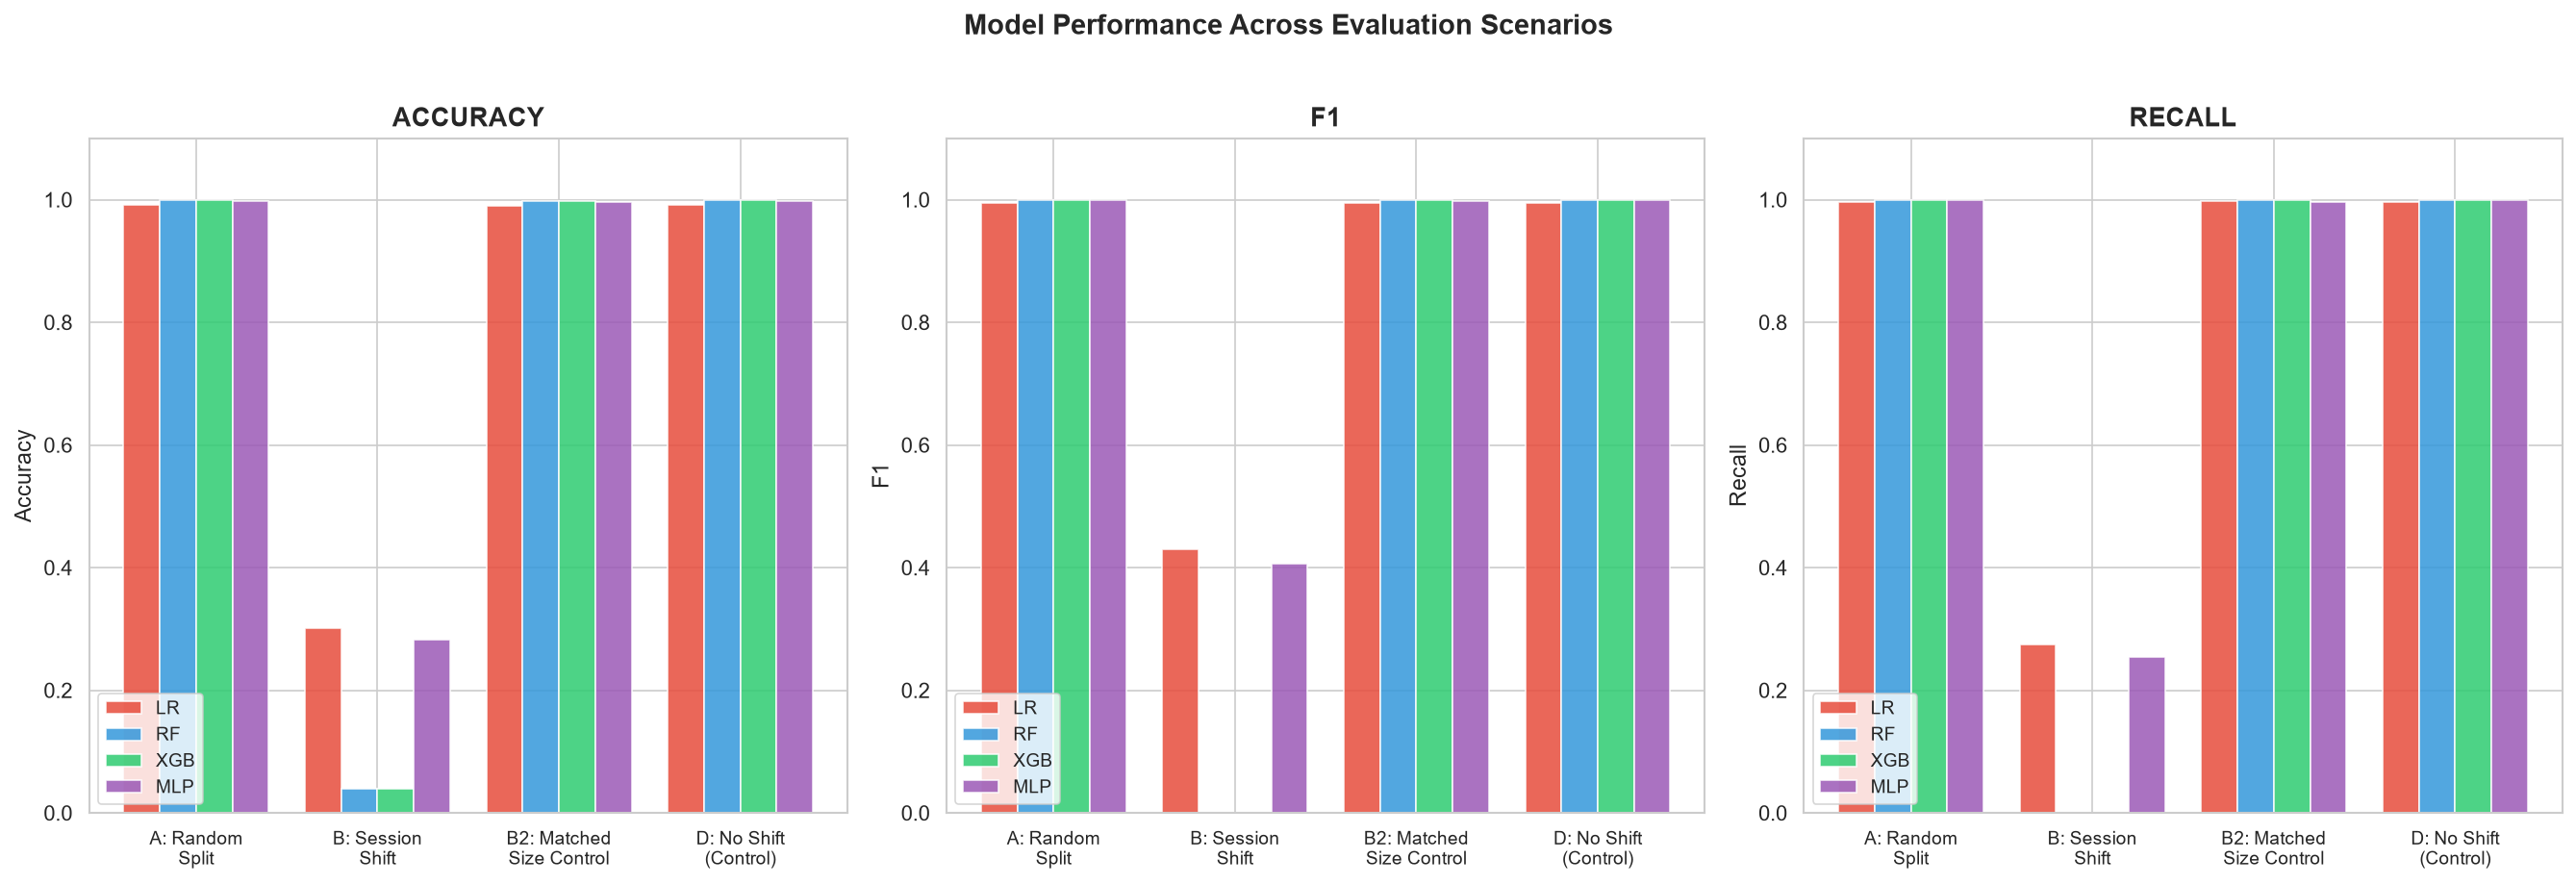
\includegraphics[width=0.9\textwidth]{fig1.png}
\caption{Model performance (accuracy, F1, recall) across the random-split, session-shift, matched-size, and no-shift evaluation scenarios.}
\label{fig:1}
\end{figure}
\begin{figure}[ht]
\centering
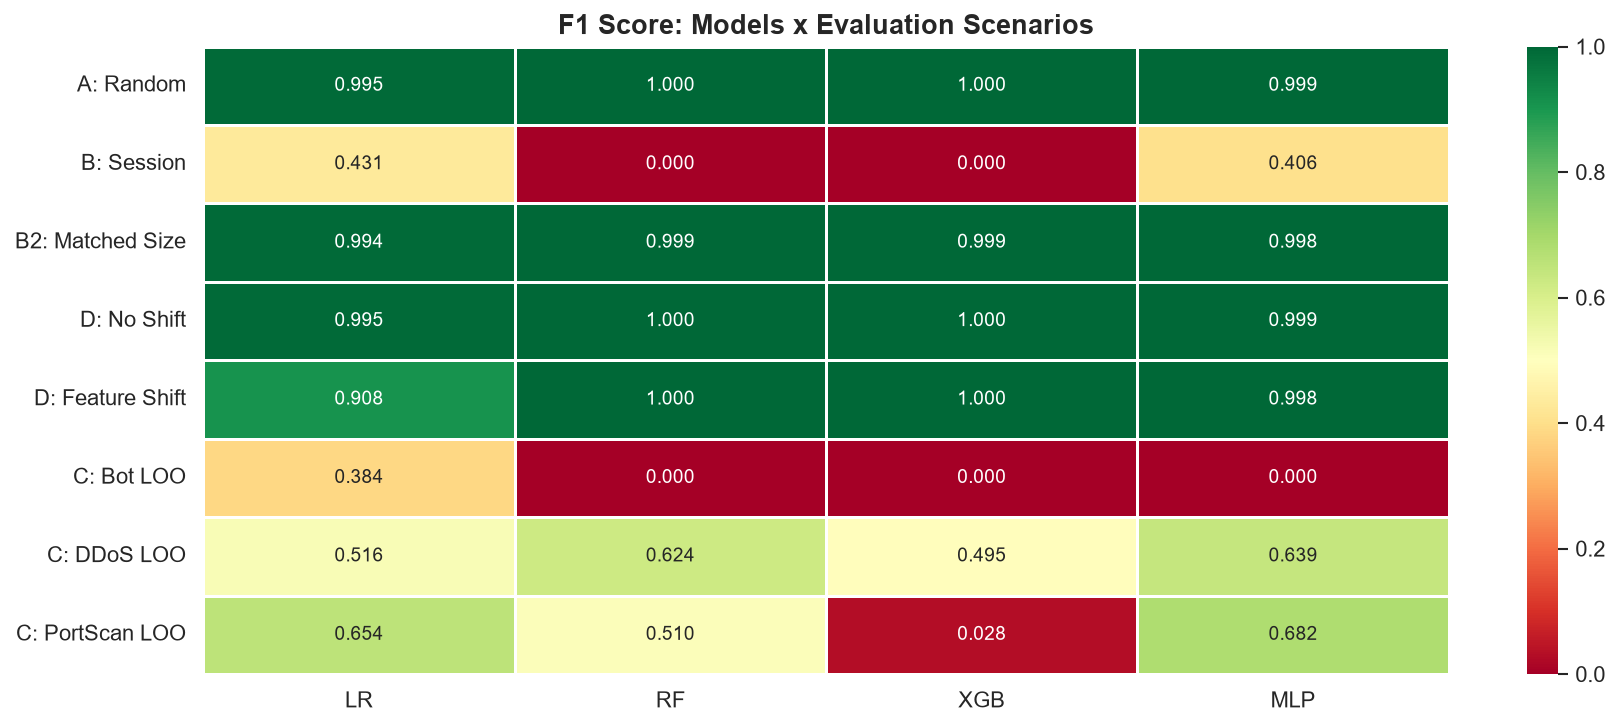
\includegraphics[width=0.9\textwidth]{fig2.png}
\caption{F1-score landscape across models and evaluation scenarios, including the attack-family leave-one-out results.}
\label{fig:2}
\end{figure}
\subsection{Joint Session and Attack-Family Shift (Experiment B)}
Under this shift, performance degrades dramatically (Table 2). Random Forest collapses to F1 = 0.0000, predicting all traffic as benign. XGBoost similarly collapses to F1 = 0.0003. Logistic Regression retains partial detection (F1 = 0.4307) and MLP limited detection (F1 = 0.4059), but both miss roughly 73\% of attacks. Since B combines unseen attack classes (DDoS, PortScan) with session-level covariate shift, Experiment B4 and the Wasserstein quantification in Section 7.7 attribute this degradation to its constituent causes.
\begin{table}[ht]
\centering
\small
\setlength{\tabcolsep}{5pt}
\caption{Experiment B results. Severe degradation, especially for tree-based models.}
\begin{tabular}{l r r r r r r}
\toprule
Model & Accuracy & F1 & Precision & Recall & FPR & Infer (ms) \\
\midrule
------- & ---------- & ----- & ----------- & -------- & ------ & ----- \\
LR & 0.3021 & 0.4307 & 0.9949 & 0.2748 & 0.0343 & 0.0001 \\
RF & 0.0393 & 0.0000 & 0.0000 & 0.0000 & 0.0040 & 0.0016 \\
XGB & 0.0395 & 0.0003 & 0.6282 & 0.0002 & 0.0025 & 0.0003 \\
MLP & 0.2833 & 0.4059 & 0.9960 & 0.2549 & 0.0249 & 0.0007 \\
\bottomrule
\end{tabular}
\end{table}
The low accuracy for RF (0.0393) and XGB (0.0395) may look paradoxical given that the test set is 96.1\% attack. It is explained by the models predicting benign for almost everything: a model that predicts all-benign on a test set that is only 3.9\% benign gets roughly 3.9\% accuracy. The low FPR values (0.0040, 0.0025) are not positive signals either. They are symptoms of total detection failure, because the models never predict attack at all.
\subsection{Isolating Distribution Shift from Train Size (B vs B2)}
The most important comparison is B against its matched-size control B2 (Table 3). Both use 13,736 training samples; the only difference is whether training data comes from the same distribution as the test set (B2) or a different one (B).
\begin{table}[ht]
\centering
\small
\setlength{\tabcolsep}{5pt}
\caption{Distribution shift isolation. B and B2 use the same training set size (13,736) with zero train/test overlap.}
\begin{tabular}{l r r}
\toprule
Model & B: Session Shift & B2: Same Distribution \\
\midrule
------- & ------------------: & ----------------------: \\
LR & 0.4307 & 0.9942 \\
RF & 0.0000 & 0.9992 \\
XGB & 0.0003 & 0.9991 \\
MLP & 0.4059 & 0.9979 \\
\bottomrule
\end{tabular}
\end{table}
The contrast is stark. With the same 13,736 training samples, RF achieves F1 = 0.9992 under same-distribution conditions (B2) but F1 = 0.0000 under distribution shift (B). This is strong evidence that the degradation is distributional, not a shortage of training data.
The implication is direct: 13,736 training samples are not insufficient. They produce near-perfect performance when they match the test distribution. The problem is that the training data, though from the same dataset, comes from sessions and attack types that do not represent the test distribution. That is a fundamentally different problem from data scarcity and needs different solutions (distribution-aware evaluation, continual retraining, or domain adaptation) rather than simply collecting more labels. Figure 3 shows this contrast directly.
\begin{figure}[ht]
\centering
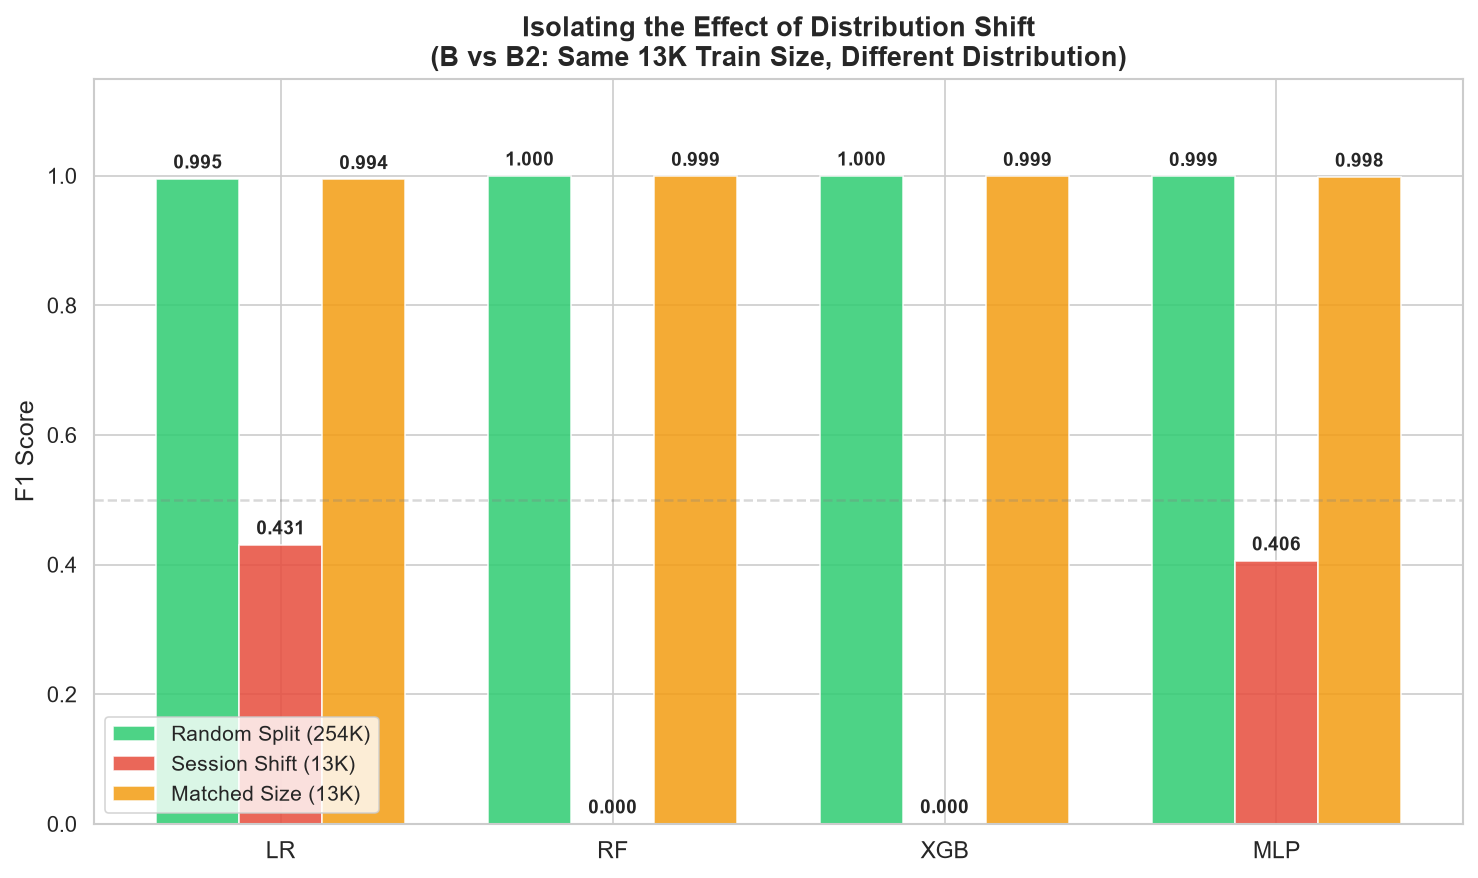
\includegraphics[width=0.9\textwidth]{fig3.png}
\caption{Isolating distribution shift from train size. B and B2 use identically sized training sets (13,736 samples) whose distributions differ.}
\label{fig:3}
\end{figure}
\subsection{Separating Unseen-Class Shift from Covariate Shift (Experiment B4)}
Experiment B's test set contains attack families absent from training, so its collapse could in principle be blamed on either novel attack signatures or displaced feature values. Experiment B4 removes the unseen-class component: DDoS is present in training, and only the test feature values are perturbed (Table 4).
\begin{table}[ht]
\centering
\small
\setlength{\tabcolsep}{5pt}
\caption{Single-class covariate-shift control. DDoS is present in both training and test; only test features are perturbed. F1 drops are negligible compared with Experiment B.}
\begin{tabular}{l r r r}
\toprule
Model & B4a: Same Dist. & B4b: Covariate Shift & Delta \\
\midrule
------- & ----------------: & ---------------------: & ------: \\
LR & 0.9990 & 0.9982 & -0.0007 \\
RF & 0.9999 & 0.9997 & -0.0002 \\
XGB & 0.9999 & 0.9997 & -0.0003 \\
MLP & 0.9998 & 0.9995 & -0.0004 \\
\bottomrule
\end{tabular}
\end{table}
When the attack class is present in training, feature displacement of the same design as Experiment D causes negligible degradation (F1 drops of 0.0002--0.0007 across all four models), in stark contrast to Experiment B, where the same models lost 0.57--0.99 F1. The dominant driver of B's collapse is therefore the presence of entirely novel attack families (unseen-class generalization) rather than feature displacement per se. The covariate-shift part of B cannot be fully separated from its class-composition change here, but B4 shows that displacement alone, even a moderate one (normalized Wasserstein 0.152, Section 7.7), does not produce B's catastrophic failures. This frames B as an open-set recognition problem: the models have no decision boundary for attack families they have never seen.
\subsection{Attack-Family Leave-One-Out (Experiment C)}
When specific attack types are excluded from training (Table 5), the results reveal which families are most distinct from the training distribution.
\begin{table}[ht]
\centering
\small
\setlength{\tabcolsep}{5pt}
\caption{F1 scores under attack-family leave-one-out. Bot detection is most severely affected.}
\begin{tabular}{l r r r r}
\toprule
Held-out & LR & RF & XGB & MLP \\
\midrule
---------- & -----: & -----: & -----: & -----: \\
Bot & 0.384 & 0.000 & 0.000 & 0.000 \\
DDoS & 0.516 & 0.624 & 0.495 & 0.639 \\
PortScan & 0.654 & 0.510 & 0.028 & 0.682 \\
\bottomrule
\end{tabular}
\end{table}
The Bot leave-one-out is the most severe: all models except LR hit F1 = 0.000 when Bot is absent from training, despite 314,325 training samples from the other three classes. Bot traffic is evidently highly distinct from DDoS and PortScan in feature space, and learned patterns do not transfer. DDoS and PortScan leave-one-out degrade more gracefully, with MLP best (0.639 and 0.682), because Bot traffic in training shares more feature overlap with these families. ``Unseen attack type'' is thus not a uniform category: some unseen attacks are more detectable, depending on their feature similarity to known attacks. Figure 4 plots the leave-one-out F1 scores; Figure 5 converts them into relative degradation from the baseline.
\begin{figure}[ht]
\centering
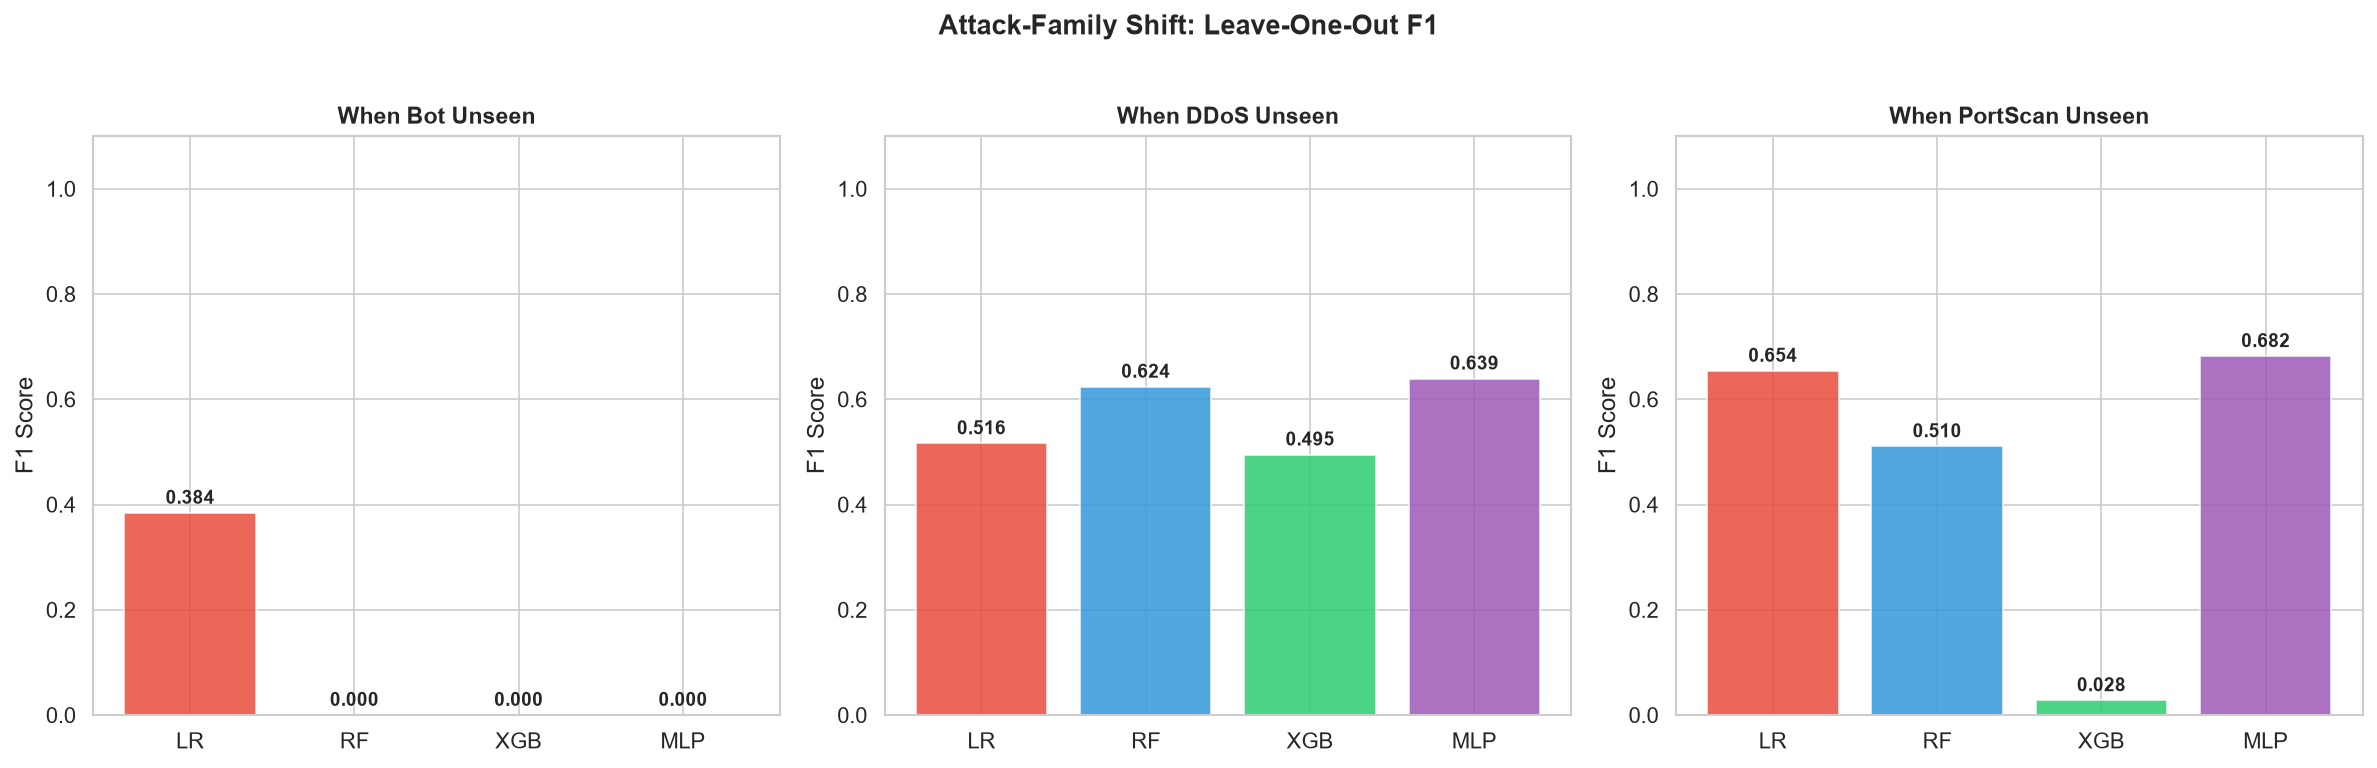
\includegraphics[width=0.9\textwidth]{fig4.png}
\caption{Attack-family leave-one-out F1 per held-out class. Bot detection is the most severely affected.}
\label{fig:4}
\end{figure}
\begin{figure}[ht]
\centering
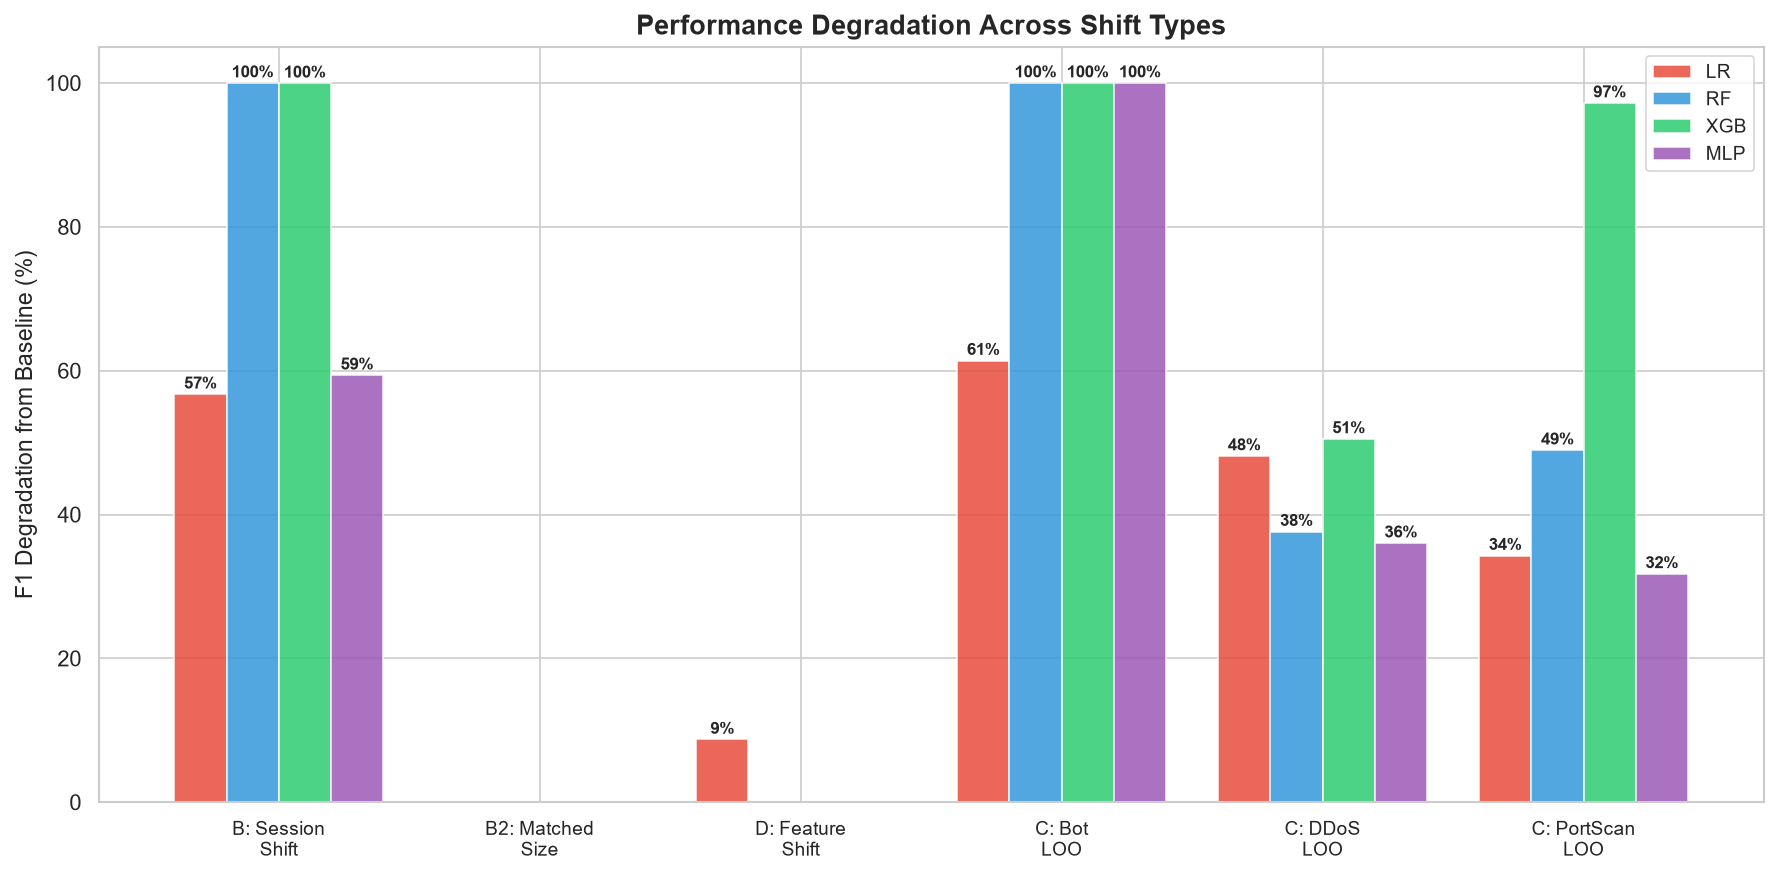
\includegraphics[width=0.9\textwidth]{fig5.png}
\caption{F1 degradation relative to the Experiment A baseline for each shift condition and model.}
\label{fig:5}
\end{figure}
\subsection{Synthetic Feature Perturbation (Experiment D)}
Under synthetic feature perturbation (Table 6), tree-based models are largely unaffected (RF and XGB both stay at F1 = 0.9997), while Logistic Regression shows clear degradation (0.9951 to 0.9084).
\begin{table}[ht]
\centering
\small
\setlength{\tabcolsep}{5pt}
\caption{Experiment D results. Tree models showed little degradation under the specific feature perturbations used in this experiment.}
\begin{tabular}{l r r}
\toprule
Model & No Shift & Feature Shift \\
\midrule
------- & ----------: & --------------: \\
LR & 0.9951 & 0.9084 \\
RF & 0.9997 & 0.9997 \\
XGB & 0.9997 & 0.9997 \\
MLP & 0.9989 & 0.9983 \\
\bottomrule
\end{tabular}
\end{table}
RF and XGBoost barely moved under this perturbation design (F1 effectively unchanged at 0.9997). This is an empirical result for this particular design, not evidence of general invariance to feature distribution changes. There is a mechanical explanation: tree models split on feature ranks and thresholds, so scaling features by positive factors does not reorder samples at a given split, leaving decision boundaries intact; linear models, by contrast, combine features additively with learned weights, so multiplying feature magnitudes directly shifts the linear scores and their calibration to the 0.5 threshold. Logistic Regression therefore degrades as expected (0.9951 to 0.9084).
The contrast is informative. Tree models were highly vulnerable to session/attack-family shift (Experiment B) but stable under this particular perturbation. More realistic perturbations, such as changed feature correlations, new features from protocol changes, or dropped features from sensor failures, could affect tree models differently.
\subsection{Shift Magnitude Quantification (Wasserstein Distances)}
The preceding experiments describe shifts qualitatively; Table 7 quantifies them. For each shift I report the mean normalized one-dimensional Wasserstein distance between training and test features (a random subsample of 25,000 points per side, per-feature distance divided by the pooled standard deviation).
\begin{table}[ht]
\centering
\small
\setlength{\tabcolsep}{5pt}
\caption{Mean normalized Wasserstein distance between training-feature and test-feature distributions, per shift, with the largest per-feature distances and the largest observed F1 drop across the four models (baseline = the experiment's own no-shift condition: random split A for B, B4a for B4, no-shift control for D).}
\begin{tabular}{l r p{4.5cm} r}
\toprule
Shift & Mean W1 (norm.) & Top shifted features & Max F1 drop \\
\midrule
------- & ----------------: & ---------------------- & ------------: \\
B (joint session + unseen class) & 0.293 & PSH Flag Count (1.01), Min Packet Length (0.81), Bwd Packet Length Min (0.77) & 0.9997 (RF) \\
B4 (seen-class covariate shift) & 0.152 & Flow Duration, packet counts (as in D) & 0.0008 (LR) \\
D (synthetic feature perturbation) & 0.106 & Packet Length Variance (0.59), Flow Duration (0.47), Flow IAT Std (0.47) & 0.0867 (LR) \\
\bottomrule
\end{tabular}
\end{table}
Three observations follow. First, B is the largest displacement (0.293) and produces the largest F1 collapse, in the expected direction. Second, the relationship between displacement and degradation is strongly non-linear: B4 displaces features roughly half as much as B (0.152 vs. 0.293) yet produces about a thousand-fold smaller F1 drop. Third, B's F1 drop of 0.9997 is far out of proportion to what feature displacement alone would predict from B4, confirming that unseen-class generalization, not covariate magnitude, is the primary driver of B's collapse. Figure 6 reports this relationship directly.
\begin{figure}[ht]
\centering
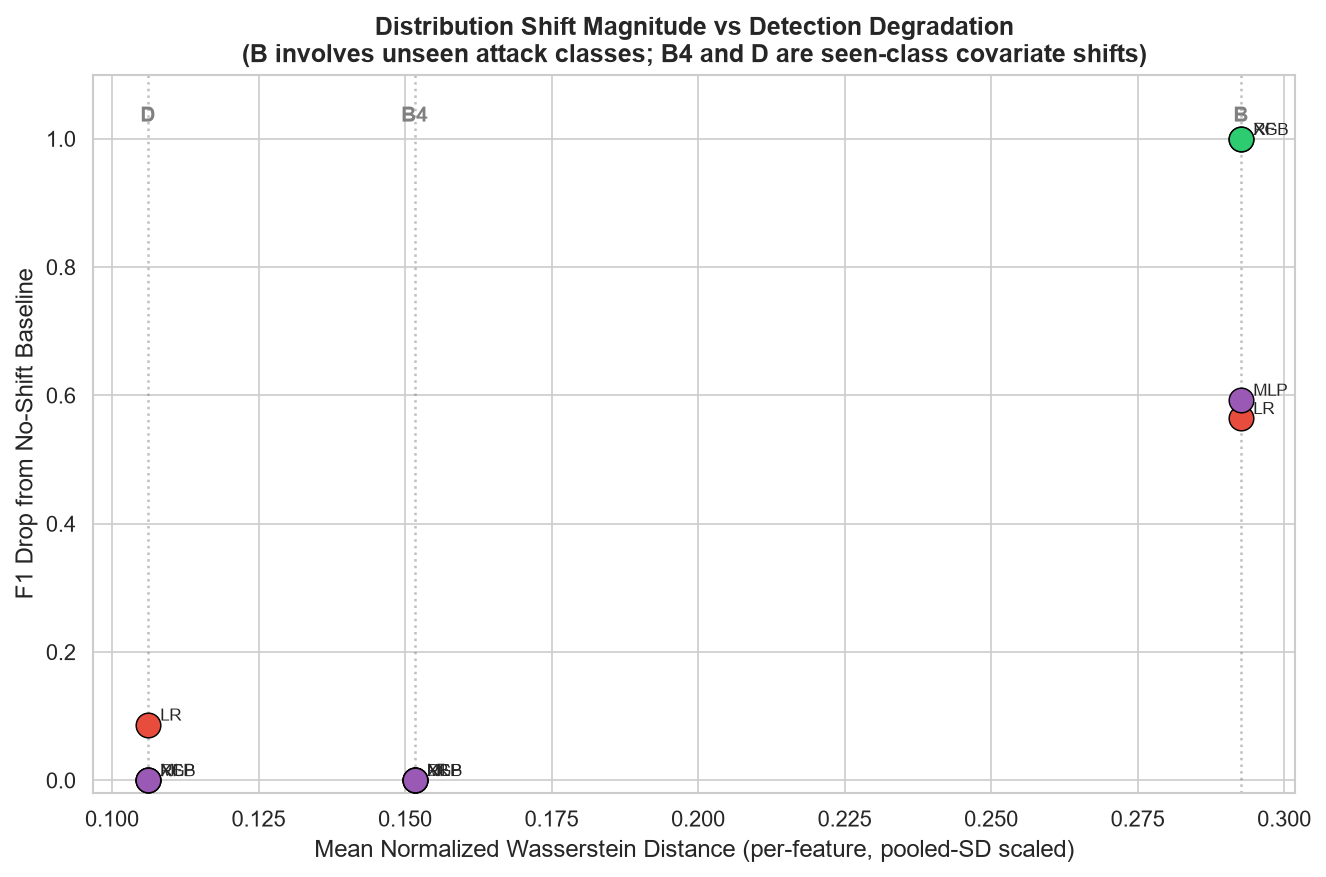
\includegraphics[width=0.9\textwidth]{fig6.png}
\caption{Mean normalized Wasserstein shift magnitude versus maximum F1 drop across the B, B4, and D shifts.}
\label{fig:6}
\end{figure}
\subsection{Threshold Sweep on the Shifted Test Set}
The ROC-AUC analysis below shows that rankings survive even when F1 collapses at the default threshold; the sweep (Section 6.5) tests whether this signal is usable. Table 8 reports F1 and FPR at the default threshold (0.50), at a moderately aggressive threshold (0.05), and at an aggressive threshold (0.01); Figure 7 shows the full curves.
\begin{table}[ht]
\centering
\small
\setlength{\tabcolsep}{5pt}
\caption{Threshold sweep on the Experiment B test set. Lowering the decision threshold recovers a substantial fraction of F1 at the cost of higher FPR; even at the best non-degenerate thresholds, all models still underperform their same-distribution baselines.}
\begin{tabular}{l r r r r r r}
\toprule
Model & F1 @ 0.50 & FPR @ 0.50 & F1 @ 0.05 & FPR @ 0.05 & F1 @ 0.01 & FPR @ 0.01 \\
\midrule
------- & ----------: & -----------: & ----------: & -----------: & ----------: & -----------: \\
LR & 0.4307 & 0.0343 & 0.7104 & 0.0581 & 0.7115 & 0.1602 \\
RF & 0.0000 & 0.0040 & 0.7114 & 0.0399 & 0.8262 & 0.0654 \\
XGB & 0.0003 & 0.0025 & 0.4635 & 0.0081 & 0.6037 & 0.0219 \\
MLP & 0.4059 & 0.0249 & 0.4923 & 0.0368 & 0.6614 & 0.0492 \\
\bottomrule
\end{tabular}
\end{table}
Threshold-based recalibration recovers part of the collapsed F1: Random Forest rises from 0.0000 (FPR 0.4\%) at the default threshold to 0.7114 at 0.05 and 0.8262 at 0.01, with FPR climbing to 4.0\% and 6.5\%. The ranking signal identified by ROC-AUC is therefore real and exploitable, but recovery is neither free nor complete. First, the required thresholds (0.01--0.05) are far below the default, so near-line-rate deployments would flag a large share of traffic; the FPR cost looks diluted on this 96.1\%-attack test set but would be far larger in benign-dominated production traffic. Second, the naive best-F1 point on this test set is the degenerate solution of predicting every sample as attack (F1 = 0.98 at FPR = 1.0), which provides no useful detection. Third, even the best recoverable operating point (RF, 0.8262) falls below same-distribution capability (B2, 0.9992): recalibration is a partial remedy, not a restoration of the original decision function.
\begin{figure}[ht]
\centering
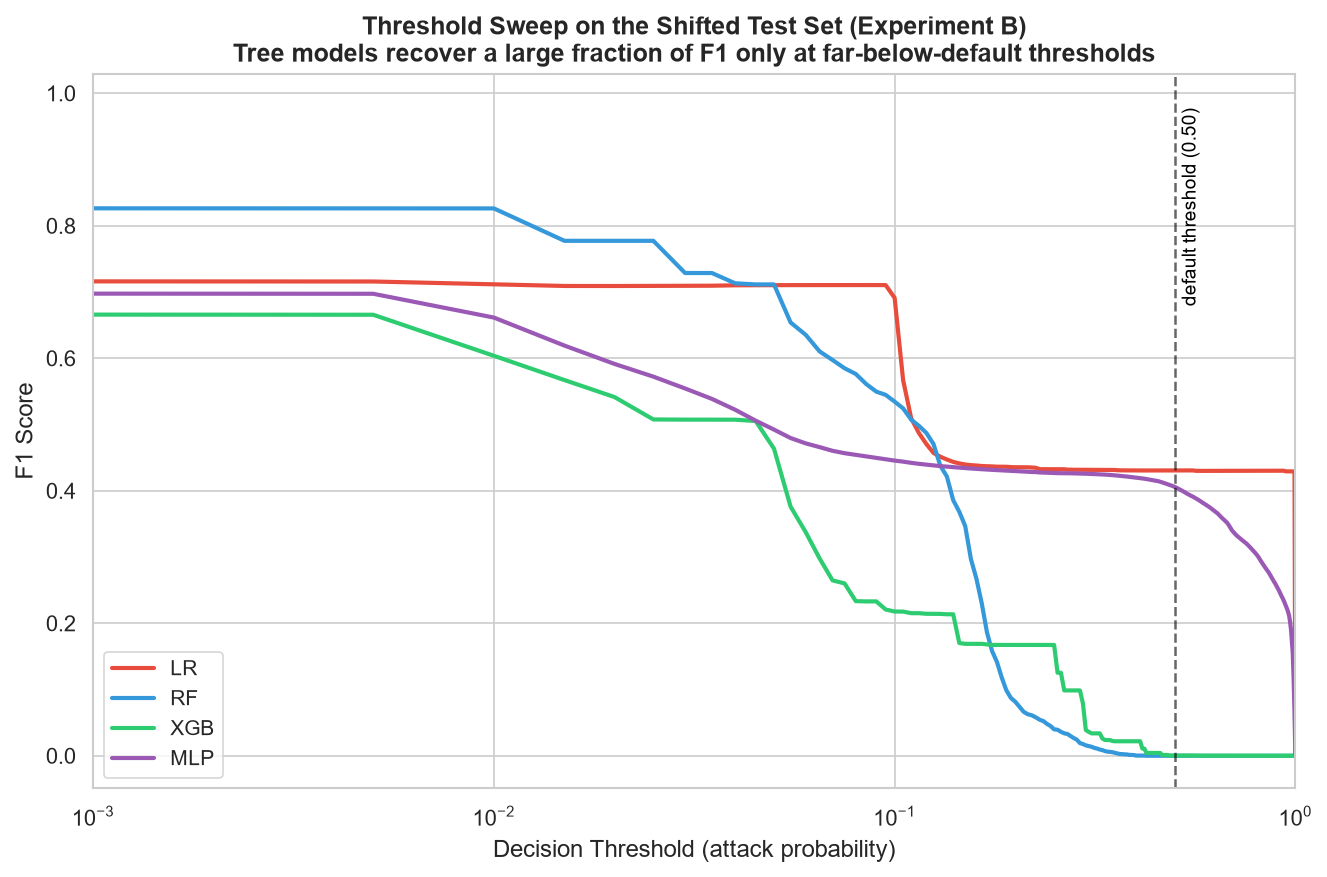
\includegraphics[width=0.9\textwidth]{fig7.png}
\caption{F1 versus decision threshold on the Experiment B test set. Tree models require far-below-default thresholds to recover useful F1.}
\label{fig:7}
\end{figure}
\subsection{ROC-AUC Under Shift}
An important secondary finding emerges from comparing F1 and ROC-AUC under session-based shift (Table 9). Figure 8 compares ROC-AUC across scenarios.
\begin{table}[ht]
\centering
\small
\setlength{\tabcolsep}{5pt}
\caption{F1 collapses while ROC-AUC retains partial signal under distribution shift.}
\begin{tabular}{l r r}
\toprule
Model & F1 (B) & ROC-AUC (B) \\
\midrule
------- & --------: & -------------: \\
LR & 0.4307 & 0.6081 \\
RF & 0.0000 & 0.8185 \\
XGB & 0.0003 & 0.8452 \\
MLP & 0.4059 & 0.6485 \\
\bottomrule
\end{tabular}
\end{table}
RF achieves ROC-AUC = 0.8185 despite F1 = 0.0000, and XGB achieves 0.8452 despite F1 = 0.0003. This suggests the models' probability rankings retain some discriminative information, while the default classification threshold is poorly suited to the shifted test distribution. In other words, the failure is one of calibration rather than of learned representations: the ranking survives, and the default operating point does not. The threshold sweep in Section 7.8 confirms this interpretation: the retained ranking signal can be converted back into classification performance, but only at far-below-default thresholds with a measurable false-alarm cost, so the recoverable signal is bounded. Monitoring ROC-AUC alongside F1 in production could provide an early-warning signal (distinguishing threshold miscalibration from fundamental model failure), but the sweep shows the practical remedy is limited.
\begin{figure}[ht]
\centering
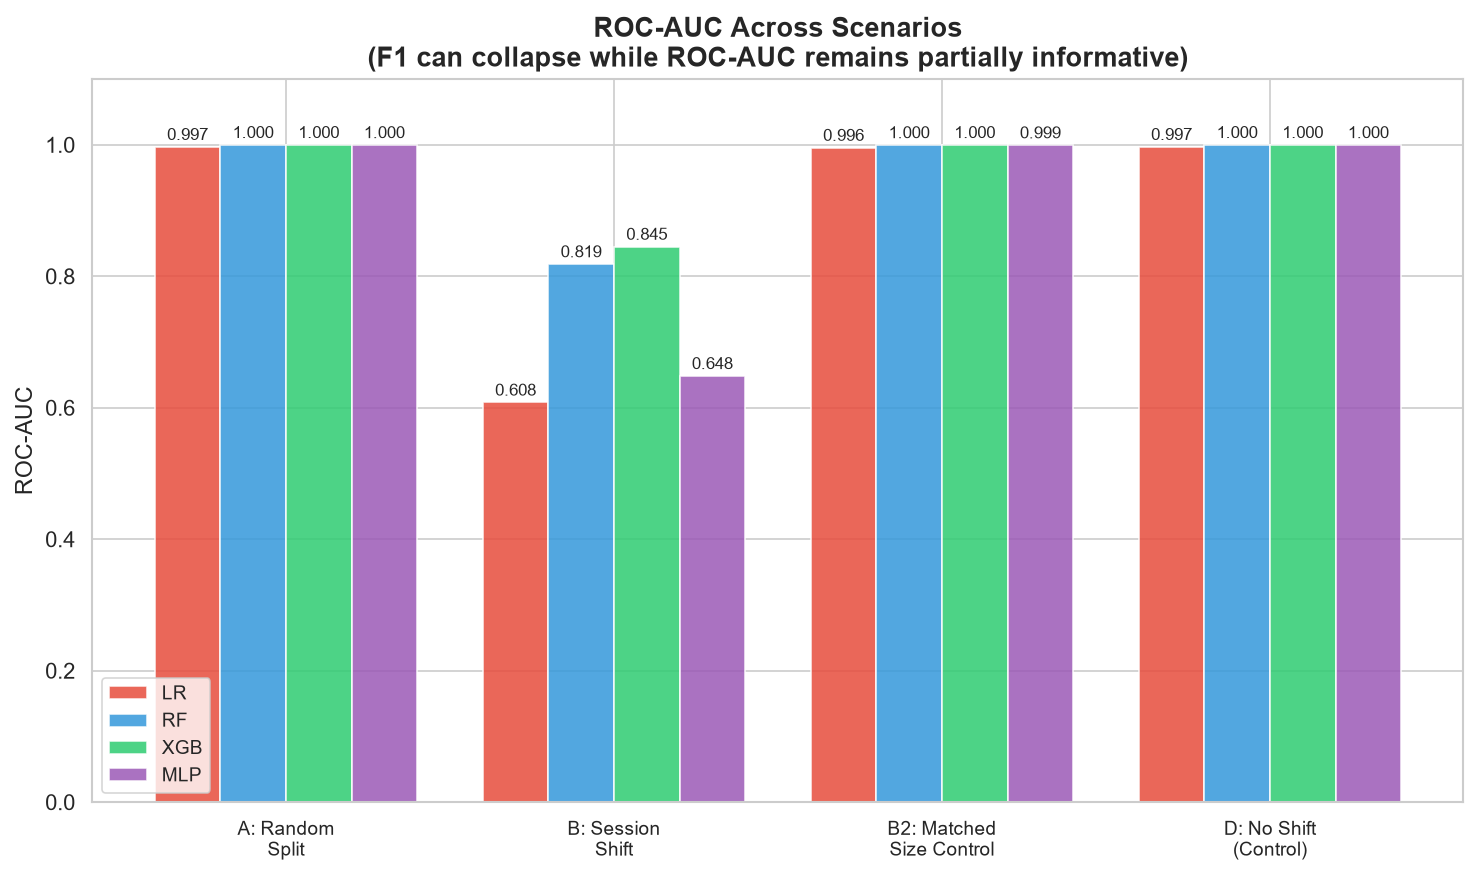
\includegraphics[width=0.9\textwidth]{fig8.png}
\caption{ROC-AUC across evaluation scenarios. F1 can collapse while ROC-AUC retains a partial ranking signal.}
\label{fig:8}
\end{figure}
\section{Security Implications}
\subsection{The False Sense of Security Problem}
The central security implication is that conventional evaluation can produce a false sense of security. A model reported as 99.97\% effective may provide zero detection capability in deployment, and this is a predictable consequence of the gap between evaluation and deployment conditions.
There is a paradox in the numbers: the models with the highest benchmark scores in this experiment (RF and XGB at 0.9997) also failed the most catastrophically under the evaluated shift. Predicting all traffic as benign means they provide no security value while appearing, by conventional metrics, to be the strongest performers. This supports the emphasis of the NIST AI Risk Management Framework and NIST IR 8596 on continuous monitoring and adaptation: a model that performs well at one point may fail in a changed environment, and standard evaluation will not detect this before deployment.
\subsection{Failure Mode Analysis}
The failure modes differ by architecture, with different security consequences:
\textbf{Tree-based models (RF, XGB):} Fail by predicting all traffic as benign (recall approaches 0). This is the worst possible failure mode: every attack passes undetected while the model projects the illusion of a clean network.
\textbf{Linear and neural models (LR, MLP):} Fail by detecting only a subset of attacks (recall approximately 0.25--0.27) with high precision. They miss roughly 73\% of attacks but rarely raise false alarms. Imperfect, yes, but this failure mode keeps at least partial visibility into threats.
From an operational standpoint, the tree-based failure mode is strictly worse: a model that never raises an alarm provides no security value, and deploying it may even increase risk by replacing signature-based systems that would have caught some attacks. The practical implication for model selection in cloud security is that \textbf{the model that performs best under conventional evaluation may not be the most robust choice for deployment.} Organizations should evaluate candidates under distribution-aware conditions before deploying rather than trusting benchmark scores alone. If only conventional evaluation is feasible, these results suggest LR or MLP showed less catastrophic degradation under the evaluated shift, despite their lower benchmark scores.
\subsection{Implications for Cloud Deployment}
Deploying ML-based intrusion detection in clouds adds complexity. In centralized architectures where traffic from multiple services is fed into a single model, the distribution shift problem is amplified. my finding that tree-based models collapse under even a single session-based shift suggests that any model expected to generalize across diverse traffic types is especially at risk.
\textbf{Inference latency.} Inference times differ by an order of magnitude (LR 0.0001 ms/sample, MLP 0.0006, RF 0.0014). At cloud scale, where millions of flow records may be classified per minute, these differences are operationally significant. But the latency advantage of LR is meaningless if the model fails to detect attacks under shift, so the speed-robustness trade-off should be informed by distribution-aware evaluation.
\textbf{Threshold sensitivity.} The threshold sweep confirms that the retained ranking signal is exploitable but bounded. All four models kept ROC-AUC well above 0.5 under shift, so an operator could recover a large fraction of F1 by lowering the threshold, but only by moving far from 0.50 (to roughly 0.01--0.05), at which point FPR and the share of flagged traffic rise materially: Random Forest's FPR increases from 0.4\% at threshold 0.50 to 6.5\% at threshold 0.01. A real deployment in benign-dominated traffic would see a proportionally larger false-alarm volume than the 96.1\%-attack test set suggests, and picking the operating threshold without ground-truth labels from the target distribution is a practical challenge.
\textbf{Hybrid architectures.} The differing failure modes across architectures suggest that ensembles mixing model types may be more robust. A system that combines tree-based models (fast inference, high benchmark performance) with linear models (graceful degradation under shift) could take the strengths of each while covering their weaknesses.
\section{Limitations}
\textbf{Dataset scope.} I use only the Friday subset of CICIDS2017 (BENIGN, Bot, DDoS, PortScan). The full dataset includes additional attack categories (Brute Force, Heartbleed, Web Attacks, Infiltration) spread across Monday through Friday, which may produce different shift patterns, and these findings may not generalize to datasets with different attack types or network configurations. Future work should replicate this analysis on UNSW-NB15, CICIDS2018, and real production traffic.
\textbf{Session-shift construction.} In Experiment B, the session-based split partitions by attack type (Bot = morning, DDoS/PortScan = afternoon). This approximates but does not perfectly replicate a pure timestamp-level temporal split, because preprocessing concatenates rows by class, partially destroying the original temporal ordering. I therefore label it \textit{session and attack-family shift} rather than \textit{temporal shift}.
\textbf{Train-test size imbalance.} The session split produces substantially different training and test set sizes (13,736 vs. 298,609). The B2 control confirms that distribution shift, not train size, is the primary cause of degradation, but the imbalance also shifts class proportions (training is 85.7\% benign; test is 3.9\% benign), which is an additional variable in the design.
\textbf{Model configurations.} I evaluate four architectures with fixed, untuned hyperparameters; other configurations might have different robustness profiles. However, the complete collapse of RF and XGB under session shift suggests the main finding is robust to moderate hyperparameter variation. I do not evaluate recurrent, attention-based, or graph-neural architectures, which may behave differently; the ML focus here is deliberate (Section 5.3).
\textbf{Feature shift design.} The synthetic perturbation in Experiment D is limited: it multiplies flow-level magnitudes by positive factors while preserving feature correlations. Tree models showed little degradation under this transformation, but that does not establish robustness to joint-distribution, correlation, feature-availability, or sensor changes, any of which could reorder samples across tree splits. Joint-distribution shifts remain untested.
\textbf{Binary classification focus.} While I report multi-class results, the primary analysis uses binary classification (BENIGN vs. ATTACK). Distribution shift may affect multi-class performance differently, especially class-specific detection.
\section{Conclusion}
The results show that conventional random-split evaluation can substantially overestimate the operational effectiveness of ML-based intrusion detection models. Models that score 0.999+ F1 on a random split collapsed to 0.000 under distribution shift, while a matched-size control trained on the same number of samples from the same distribution held at 0.999. The gap is distributional, not a shortage of training data.
The failure modes differ by architecture in ways that have direct security implications. Tree-based models, which earn the highest benchmark scores, fail the most catastrophically (complete detection collapse), while linear and neural models retain partial detection. The single-class covariate-shift control shows that feature displacement on a seen class is comparatively benign, attributing the collapse in the joint session/attack-family scenario primarily to unseen attack classes rather than covariate magnitude. The secondary finding that ROC-AUC stays partially informative while F1 collapses suggests the models retain discriminatory information despite broken operational behavior; a threshold sweep confirms this signal can be partially recovered, but only at far-below-default thresholds whose false-alarm cost must be borne in benign-dominated deployment traffic.
These findings have implications for both research methodology and operational deployment. For researchers, the results support distribution-aware evaluation as a complement to conventional benchmarking: random-split evaluation remains a useful upper bound on capability, but it should not be the only methodology. Any study reporting high performance on an IDS benchmark should supplement random-split results with at least one distribution-shift evaluation. For practitioners, the results caution against relying on benchmark performance alone when choosing deployment models: organizations should evaluate candidates under conditions matching their deployment environment, monitor for distribution drift in production, keep fallback detection mechanisms independent of ML assumptions, and set up retraining protocols that account for how traffic and attack patterns evolve over time.
Several directions for future work emerge. First, the framework should be replicated on additional datasets (UNSW-NB15, CICIDS2018) and architectures (recurrent networks, transformers, and calibrated variants such as Platt-scaled or isotonic-regression classifiers). Second, distribution shift detection methods that alert operators when operating conditions diverge from training conditions would complement robustness evaluation, with the ROC-AUC-versus-F1 gap identified here as a candidate early-warning signal. Third, domain adaptation and continual learning approaches that address shift during deployment could offer more robust alternatives to static deployment. Fourth, adaptive threshold strategies informed by the sweep results (including operating-point selection that accounts for false-alarm cost in benign-dominated traffic) could operationalize the ROC-AUC finding.
The broader lesson is that evaluation methodology itself shapes the conclusions I draw about model capability: a model evaluated under conditions that do not match deployment is effectively a different model. As ML-based intrusion detection matures, standardized robustness evaluation protocols (analogous to adversarial robustness benchmarks in computer vision) become increasingly important for closing the gap between benchmark performance and operational security. The framework presented here, combining distribution-shift evaluation with matched-size and covariate-shift controls, Wasserstein quantification, and failure mode analysis, provides a template for such protocols.
\section*{Declarations}
\textbf{Author contributions:} Dhansika.R is the sole author: conceptualization, research direction, dataset selection, experimental design decisions, results review and interpretation, and writing.
\textbf{Use of Generative AI and AI-Assisted Technologies:} Generative AI tools were used as guided assistance throughout this project. The author conceived the research direction, selected the dataset, and made all high-level experimental design decisions in collaboration with the AI assistant tool \textit{opencode}, including the matched-size control (B2) that isolates distribution shift from training set size and the covariate-shift control (B4) that separates unseen attack classes from feature displacement. The author directed the experiments, reviewed every result, and verified the reported metrics against the experiment logs. AI assistance was used to draft the Python experiment scripts, generate the figures, and edit and polish the manuscript prose; all findings were reviewed and validated by the author, who takes full responsibility for the scientific validity and integrity of this work.
\textbf{Data and code availability:} All code (preprocessing, experiments, verification, and figure generation) and the publicly available CICIDS2017 dataset (Sharafaldin et al., 2018) are available from the author on request. The preprocessing pipeline is fully scripted and reproducible.
\textbf{Competing interests:} The author declares no competing interests.
\textbf{Funding:} This research received no specific grant from any funding agency.
\section*{References}
\begin{thebibliography}{99}
\bibitem{ref:1} Ahmad, Z., Shahid Khan, A., Wai Shiang, C., Abdullah, J., \& Ahmad, F. (2021). Network intrusion detection system: A systematic study of machine learning and deep learning approaches. \textit{Transactions on Emerging Telecommunications Technologies}, 32(1), e4150.
\bibitem{ref:2} Akinola, O., Gber, T. E., Oluwadare, T., \& Yoshida, M. (2022). Adaptive intrusion detection systems: A comprehensive review of approaches, challenges, and evaluation methodologies. \textit{Sensors}, 22(15), 5775.
\bibitem{ref:3} Coronges, K., et al. (2024). A comprehensive survey of adversarial machine learning in network intrusion detection systems. \textit{arXiv preprint}.
\bibitem{ref:4} Geirhos, R., et al. (2020). Shortcut learning in deep neural networks. \textit{Nature Machine Intelligence}, 2(11), 665--673.
\bibitem{ref:5} Nibouchia, O., et al. (2024). Temporal evaluation in intrusion detection: A systematic literature review. \textit{Computers \& Security}, 137, 103551.
\bibitem{ref:6} NIST. (2023). AI Risk Management Framework (AI RMF 1.0). National Institute of Standards and Technology.
\bibitem{ref:7} NIST. (2025). NISTIR 8596: Cybersecurity Framework Profile for Artificial Intelligence. National Institute of Standards and Technology.
\bibitem{ref:8} Sadhnani, M., et al. (2024). Explainable AI for concept drift detection in network intrusion detection systems. \textit{Computers \& Security}, 137, 103568.
\bibitem{ref:9} Sharafaldin, I., Lashkari, A. H., \& Ghorbani, A. A. (2018). Toward generating a new intrusion detection dataset and intrusion traffic characterization. \textit{Proceedings of ICISSP}, 108--116.
\bibitem{ref:10} Shyaa, S. H., et al. (2024). Concept drift in intrusion detection: A comprehensive survey. \textit{IEEE Access}, 12, 45000--45025.
\bibitem{ref:11} Tavallaee, M., Bagheri, E., Lu, W., \& Ghorbani, A. A. (2009). A detailed analysis of the KDD CUP 99 data set. \textit{Proceedings of IEEE Symposium on Computational Intelligence for Security and Defense Applications}, 1--6.
\bibitem{ref:12} Xu, C., et al. (2024). Adversarial machine learning in intrusion detection systems: A comprehensive survey. \textit{ACM Computing Surveys}, 56(2), 1--36.
\end{thebibliography}
\end{document}
